\section{Vytvorenie vlastnej hry}\label{vytvorenie-vlastnej-hry}
Okrem zakúpenia herných titulov, vytvorených pre vzdelávacie účely, si môžu študenti vytvárať aj vlastné hry.
Tento prístup má niekoľko výhod: 
	\begin{itemize}
		\item je aplikovateľný na širokú škálu ľudí a to s rôznymi úrovňami vedomostí
		\item ušetrenie finančných zdrojov, ktoré sú inak potrebné na kúpu herného titulu
		\item zlepšenie schopnosti spolupráce a rozdelenie jednotlivých úloh pri tímových úlohách 
	\end{itemize}
V tejto sekcii sa budem zameriavať hlavne na študentov stredných škôl.\\
Proces tvorby hry od návrhu až po vývoj pozostáva z rôznych úrovní, ktorými si musí jej tvorca prejsť.
Proces zadania hry by som rozdelil do dvoch hlavných častí:
	\begin{enumerate}
		\item \textbf{Analýza zadania a základných požiadaviek pre hru.}
		\item \textbf{Implementácia zadania.}
	\end{enumerate}

	% \subsection{Edukačné ciele zadania} 
	% Zadanie by malo byť tvorené

	\subsection{Analýza zadania a základných požiadaviek zadania.}\label{analyza-zadania}
	Cieľom analýzy základných požiadaviek zadania by malo byť porozumenie 
	daný požiadavkám a vyjasnenie si prípadných nejasností v zadaní. Analýza požiadaviek 
	hry sa môže skladať z na kreslenia základného diagramu požiadaviek,
	ktoré budeme musieť hra spĺňať pri práci v tíme. Pri analýze je taktiež potrebné komunikovať 
	s vyučujúcim o požiadavkách zadania.


	\subsection{Implementácia zadania}\label{implementacia-zadania}
	\begin{enumerate}
		\item Analýza zadania hry
		\item Vytvorenie dokumentácie hry
		\item Popísanie jednotlivých scenárov
	\end{enumerate}

	\begin{figure}
		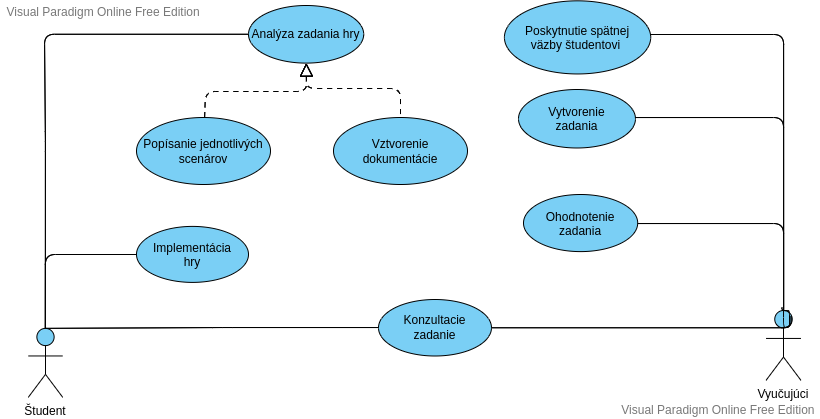
\includegraphics[width=\linewidth]{use-case.png}
		\caption{Use case diagram}
		\label{use-case-tvorba-hry}
	\end{figure}

